\documentclass[letterpaper,12pt,DIV=calc,titlepage=true,twocolumn,twoside=true,abstract=true]{scrartcl}
\let\tmp\oddsidemargin
\let\oddsidemargin\evensidemargin
\let\evensidemargin\tmp
\reversemarginpar
\usepackage[USenglish]{babel}
\usepackage[backend=biber,style=ieee,citestyle=numeric-comp]{biblatex}
\usepackage{csquotes}
\addbibresource{references.bib}
\usepackage{datetime}
\newdateformat{monthyeardate}{%
    \monthname[\THEMONTH] \THEYEAR}
\usepackage{graphicx}
\usepackage{booktabs}
\usepackage{amsmath}
\usepackage{amssymb}
\usepackage{microtype}
\PassOptionsToPackage{hyphens,spaces,obeyspaces}{url}
\usepackage[colorlinks=true]{hyperref}
\usepackage{cleveref}

\begin{document}

\title{Applications of Geospatial Data in Digital Communication}
\author{William Svoboda\\Advisor: Michael Freedman\\Department of Computer Science, Princeton University}
\date{\monthyeardate\today}

\maketitle

\begin{abstract}
    The use of geospatial data has become increasingly prevalent in digital communication. However, the core functionality of existing platforms remains largely independent of our physical surroundings. This paper presents a proof of concept for a novel communication app that uses geospatial data to control access to the sending and receiving of messages. The implications of this technology are explored, and an evaluation of the project with real users is discussed.
\end{abstract}
\cleardoubleemptypage

\section{Introduction}

With roughly 4.5 billion users worldwide~\cite{umaine_2021}, the scale of social media is testament to the importance of digital communication today. At the same time, humans are social animals. It is here in the physical world that we spend most of our time and have our closest interactions with each other. While 99\% of users access social media through mobile devices~\cite{umaine_2021}, our interaction with these services is often still independent of the physical space around us.

Previous work~\cite{ducheneaut_2006} also suggests that digital interaction does not necessarily correspond to an improved social experience. This is especially interesting in light of the ongoing \textsc{COVID-19} pandemic and the move towards remote work. Research~\cite{bonsaksen_2021,mann_2003} points to a reliance on digital communication and social media as increasing social isolation.

There is much potential, however, in exploring the intersection between digital communication and physical space. Facebook, Twitter, and Instagram—among the largest social media platforms~\cite{umaine_2021}—now incorporate geospatial data into their products. Other platforms, like Yik Yak~\cite{yikyak_2015}, even place location at the core of the user experience.

The goal of this paper is to explore how geospatial data affects our perception of digital communication. My hypothesis was that tying interaction to physical proximity using would increase user engagement. To this end, I present a novel communication app that gates the sending and receiving of messages to the user's location.

\section{Background}
\section{Related Work}

\subsection{Geocaching}

Geocaching is one of the most popular activities that centers around the use of geospatial data. Participants search for hidden caches by using \textsc{GPS}, attempting to be the first to reach a given cache's location. The coordinates for the cache, as well as clues regarding its surroundings, are posted online by organizers beforehand~\cite{natgeo_2017} and can be freely discussed. A similar activity, called waymarking, exists that actually forgoes an actual physical object. The goal instead is to reach a \enquote{virtual cache} that represents an interesting trail, vista, or other location of interest~\cite{natgeo_2017}.

\subsection{Social Media}

As previously discussed, a number of existing social media platforms already use geospatial data. The extent and purpose of geospatial data varies heavily between different services.

\subsubsection{Instagram}

Instagram is a photo and video sharing platform that was acquired by Facebook, Inc. (now Meta) in 2012. Like Facebook, Instagram uses geospatial data in the form of geotagging, where geographic information is attached as metadata. Users who click or search for a location can view a feed of other content that was posted nearby. In other words, geospatial data is used to categorize and offer additional context to user content.

\subsubsection{Twitter}

Similarly to Instagram, Twitter supports geotagging. However, this metadata is limited to images that users attach to Twitter messages, or \enquote{Tweets.} Twitter is also unique in that Tweets are limited in length and are by default text-only~\cite{twitter_2022}.

\subsubsection{Snapchat}

Snapchat is an instant messaging service focusing on \enquote{Snaps.} Snaps are photo, video, or text messages that by default last only 24 hours. Snapchat supports geotagging for both photo and video messages, and—unique to the platform—also allows messages to be sent to the app's \enquote{Snap Map} service. Snap Map, developed by Mapbox, shows a real-time heatmap of user activity overlaid on the world map~\cite{tadesse_2017}. By tapping on part of the map, users are shown a feed of Snaps posted at that location.

\subsubsection{Yik Yak}

Of the platforms that have already been mentioned, Yik Yak is the only service that actually controls access to content using geospatial data. Yik Yak is a messaging app where individual posts, called \enquote{Yaks,} are submitted and viewed within a 5-mile radius~\cite{yikyak_2015}. This gates user interaction to the immediate community surrounding them.

\section{Approach}

The design of a product straddles two distinct areas. The first, and most important, is the intended user experience. In order to evaluate my hypothesis, it was necessary to determine what features might be able to produce the desired user behavior. A large part of this process involved deciding how my project would both draw from and differentiate itself from existing platforms. Ultimately, I envisioned an application with the following qualities:

\begin{enumerate}
    \item A main screen showing the user's current location overlaid on a map of the surrounding area
    \item The ability to leave messages tied to one's location, viewable by other users and disappearing after 24 hours
    \item The restriction that a message can only be viewed when near the coordinates where it was posted
\end{enumerate}

I drew direct inspiration from Snapchat and Yik Yak in several regards. The idea of a main map screen, similar to Snap Maps, was intended to center the user experience to the world around them. Likewise, the ephemeral nature of messages mimics how individual Snaps last for only a day. The intended effect of this aspect was to keep any message encountered in the world temporally relevant. Because messages are tagged to a physical location they are also spatially relevant in the way Yik Yak messages are.

The defining characteristic of my app, however, is that access to messages is directly gated to physical proximity. While Snap Maps allows users to view Snaps anywhere on the map, and Yik Yak reveals any message sent within 5 miles, my app requires users to be almost within sight of where a message was posted in order to interact with it. My goal was that this requirement would better connect users with the messages they found by placing them in the same geospatial context.

The second area of design relates to the actual implementation of the product. Given the dominance of mobile devices in social media~\cite{umaine_2021}, I decided on an iPhone app as primary interface. This had the added benefit of access to \textsf{MapKit}, Apple's framework for geographic visualization. The actual application follows a distributed client-server model. The iPhone app, acting as the client, handles direct user interaction and communication with the server. In turn, the server handles user content, authentication, geospatial queries, and other centralized functionality.

\section{Implementation}

The client and server applications were functionally structured as two separate projects, each version controlled with \textsf{git} and hosted online with GitHub.  

\subsection{Client}

Following previous discussion, the choice of a mobile app still left the question of the exact implementation. Because I would be using \textsf{MapKit}, a native iOS application was a natural fit. The app was coded in Swift, a programming language developed by Apple explicitly for native application development on Apple hardware. This was paired with \textsf{SwiftUI}, a new framework also developed by Apple for building user interfaces. Swift and \textsf{SwiftUI} have, respectively, the benefit of interoperability with Objective-C, Apple's earlier programming language, and existing Apple interface frameworks like \textsf{UIKit}.

\textsf{SwiftUI} is a declarative framework, meaning that the user interface is simply described by the developer. This description is then translated by \textsf{SwiftUI}'s layout engine at compile-time~\cite{apple_2022}. As a result, most of the presentation logic is actually handled by the framework itself.

\subsubsection{Interface Design}

Before any code could be written, however, it was necessary to determine the general design of the user interface and the desired user flow. I wireframed the user interface using \textsf{Excalidraw}, a free and open-source tool for diagram sketches. Each screen in the wireframe was then ultimately translated into a \textsf{SwiftUI} view. \cref{fig:screenshot} demonstrates the final appearance of the app after implementation.

\begin{figure}
    \centering
    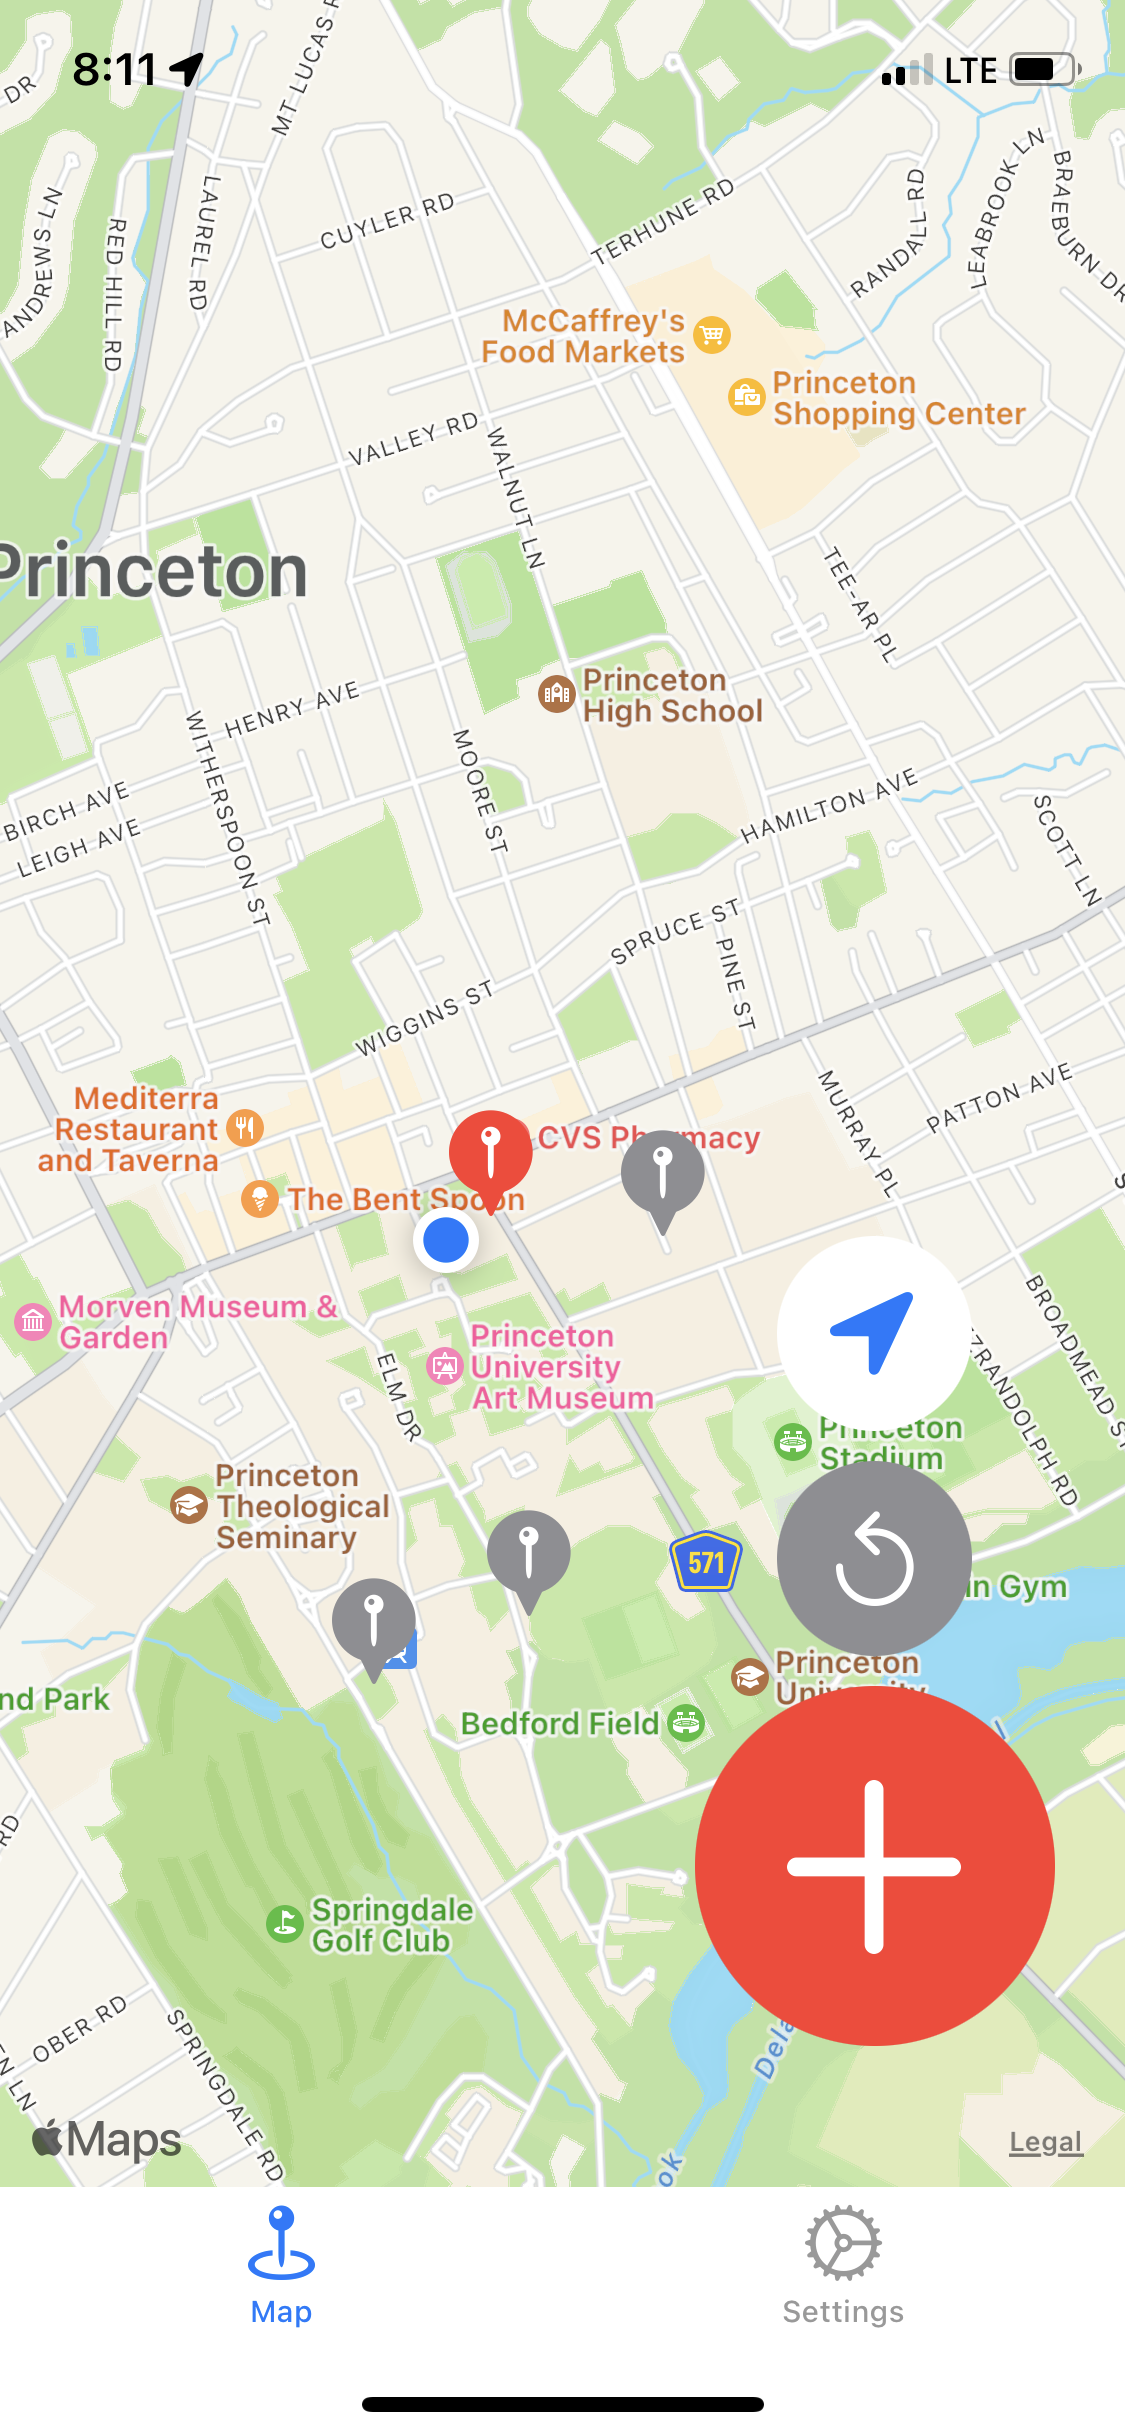
\includegraphics[width=0.5\linewidth]{screenshot.png}
    \caption{Screenshot of the main map screen}
    \label{fig:screenshot}
\end{figure}

\subsubsection{Application Architecture}

The use of \textsf{SwiftUI} naturally separates layout and appearance from the actual business logic of an app. From this, I chose the Model-View-ViewModel (\textsc{MVVM}) pattern as the underlying architecture. \textsc{MVVM} decouples presentation logic (\emph{views}) from business logic (\emph{models}) by using intermediate objects called \emph{view models}. The state of each view is bound to the associated view model, which facilitates interaction with models and user input~\cite{britch_2021,hudson_2019}.

Each part of the final user interface is composed of one or more \textsf{SwiftUI} views, with view models being used as necessary to handle state management and any dynamic behavior. In any application, it is likely certain logic needs to be shared throughout the overall system. My app needed to access global settings, authentication state, and location services at multiple points. To solve this problem, I wrote different \emph{managers} that represented a shared service layer. When required, these managers were injected into a view model to access the appropriate services.

\subsection{Server}

Compared to the client app, the server required drastically fewer lines of code. However, the difficulty was in composing the separate technologies that made up the server's basic functionality. The core \textsc{API} is handled by \textsf{FastAPI}, a high-performance web framework written in Python. I chose Redis, an in-memory datastore, as the database for its ease-of-use and included geospatial capabilities.

These core services are packaged together as one Docker application. Docker is used to containerize the server, which isolates the app from its environment. By using Docker, I could develop, test, and deploy the server on different machines while ensuring that each build would behave the same.

\subsection{Deployment}

In order to distribute the client app to users, I relied on Apple's TestFlight service. TestFlight allows developers to beta-test their iOS applications and receive feedback from users. The benefit of this approach was that I did not have to go through the full App Store approval process in order to deliver my app to testers.

The server was deployed on a DigitalOcean Droplet. Each Droplet is a Linux virtual machine (\textsc{VM}) that runs on virtualized hardware. After reserving an instance, I could access the Droplet remotely using \textsc{SSH} and install all required code and tools using \textsf{git} and the system package manager.

\section{Evaluation}
\section{Conclusions}

The application of geospatial data in digital communication remains a relatively unexplored area. It is still mostly a tool for contextual analysis or—as in social media—the organization of existing user content. This paper shows the potential of geospatial data as a means to connect users with both digital platforms and the world around them in new and interesting ways.

\subsection{Future Work}

In spite of these conclusions, there is much more that can still be done. This project is ultimately a proof of concept for the user experience I originally envisioned. There is room to flesh out the application, both client and server, to match the feature quality of commercial products. In particular, there is much potential in improving the app's interactivity beyond leaving and viewing messages. A system to add comments to an existing message, for example, would enable users to continue the conversation and facilitate interaction between users and not just with the message itself.

\printbibliography

\end{document}
